\section{Resolution Effects} \label{sec:res}

Figure demonstrating imprint SFR=0 leave on the observable space and 

how we deal with them so we can ignore them...

\begin{figure}
    \begin{center}
        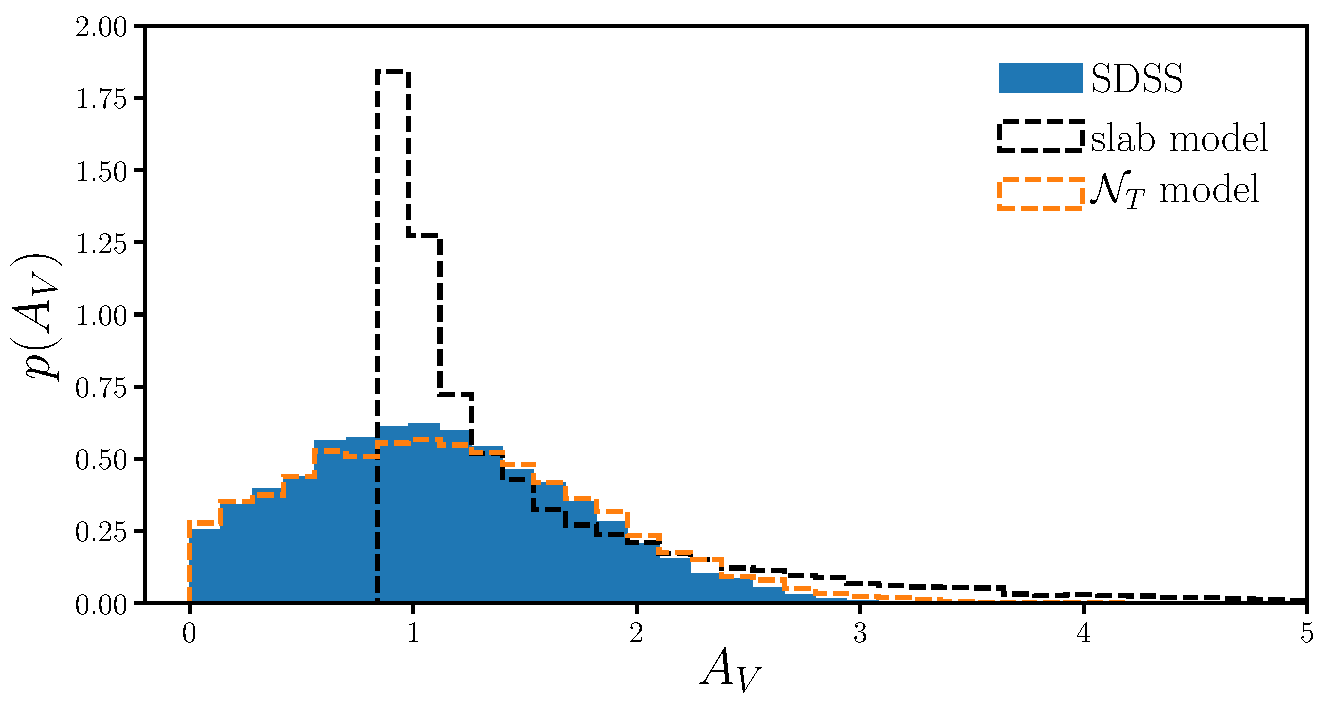
\includegraphics[width=0.66\textwidth]{figs/slab_tnorm.pdf} 
        \caption{Comparison of $A_V$ distribution of SDSS star-forming
        galaxies (blue) to predictions from the slab model (Eq.~\ref{eq:slab};
        black). {\color{red} detail on how SDSS SF galaxies are classified.} 
        The slab model assumes that there's a slab of dust in front of a galaxy.
        We use $\tau_V=2$ for the slab model above. Regardless of $\tau_V$,
        however, the slab model predicts a significantly more asymmetric and peaked $A_V$ distribution
        than observations. Given this disagreement, {\em we include in our
        analysis a DEM with an empirical prescription for $A_V$ based on a truncated normal 
        distribution, which better reproduce the observed $A_V$ distribution} (Section~\ref{sec:nonslab}). }
        \label{fig:av_dist}
    \end{center}
\end{figure}

